%%%%%%%%%%%%%%%%%%%%%%%%%%%%%%%%%%%%%%%%%
% Beamer Presentation
% LaTeX Template
% Version 1.0 (10/11/12)
%
% This template has been downloaded from:
% http://www.LaTeXTemplates.com
%
% License:
% CC BY-NC-SA 3.0 (http://creativecommons.org/licenses/by-nc-sa/3.0/)
%
%%%%%%%%%%%%%%%%%%%%%%%%%%%%%%%%%%%%%%%%%

%----------------------------------------------------------------------------------------
%	PACKAGES AND THEMES
%----------------------------------------------------------------------------------------

\documentclass[9pt, xelatex]{beamer}

\mode<presentation> {

% The Beamer class comes with a number of default slide themes
% which change the colors and layouts of slides. Below this is a list
% of all the themes, uncomment each in turn to see what they look like.


%\usetheme{default}
%\usetheme{AnnArbor}
%\usetheme{Antibes}
%\usetheme{Bergen}
%\usetheme{Berkeley}
%\usetheme{Berlin}
\usetheme{Boadilla}
%\usetheme{CambridgeUS}
%\usetheme{Copenhagen}
%\usetheme{Darmstadt}
%\usetheme{Dresden}
%\usetheme{Frankfurt}
%\usetheme{Goettingen}
%\usetheme{Hannover}
%\usetheme{Ilmenau}
%\usetheme{JuanLesPins}
%\usetheme{Luebeck}
%%\usetheme{Madrid}
%\usetheme{Malmoe}
%\usetheme{Marburg}
%\usetheme{Montpellier}
%\usetheme{PaloAlto}
%\usetheme{Pittsburgh}
%\usetheme{Rochester}
%\usetheme{Singapore}
%\usetheme{Szeged}
%\usetheme{Warsaw}

% As well as themes, the Beamer class has a number of color themes
% for any slide theme. Uncomment each of these in turn to see how it
% changes the colors of your current slide theme.

%\usecolortheme{albatross}
%\usecolortheme{beaver}
%\usecolortheme{beetle}
%\usecolortheme{crane}
%\usecolortheme{dolphin}
%\usecolortheme{dove}
%\usecolortheme{fly}
%\usecolortheme{lily}
%\usecolortheme{orchid}
%\usecolortheme{rose}
%\usecolortheme{seagull}
%\usecolortheme{seahorse}
%\usecolortheme{whale}
%\usecolortheme{wolverine}
\bibliographystyle{plain} %abbrvnat
\usepackage{natbib}
\usepackage{epstopdf}
\usepackage{graphicx} % Allows including images
\usepackage{booktabs} % Allows the use of \toprule, \midrule and \bottomrule in tables
\usepackage{amsmath} 
\usepackage{amssymb}
\usepackage{multirow}
\usepackage{amsthm}
\usepackage {tikz}
%\usepackage{tkz-graph}
\usepackage {xcolor}
\definecolor {processblue}{cmyk}{0.96,0,0,0}
\usepackage{CJKutf8}
\usepackage[cjk]{kotex}

%\setbeamertemplate{footline} % To remove the footer line in all slides uncomment this line
\setbeamertemplate{footline}[page number] % To replace the footer line in all slides with a simple slide count uncomment this line
\setbeamertemplate{caption}[numbered]
\setbeamertemplate{itemize item}[ball] % To remove the navigation symbols from the bottom of all slides uncomment this line
}


%----------------------------------------------------------------------------------------
%	TITLE PAGE
%----------------------------------------------------------------------------------------

\title[Short title]{Generalized Linear Mixed Models \\ 일반화선형혼합모형} % The short title appears at the bottom of every slide, the full title is only on the title page

\author{이소연, 황서진} % Your name
\institute[] % Your institution as it will appear on the bottom of every slide, may be shorthand to save space
{
	고려대학교 통계학과 % Your institution for the title page
\medskip
}
\date{April 8, 2021} % Date, can be changed to a custom date

\begin{document}

\begin{frame}
\titlepage % Print the title page as the first slide
\end{frame}

\begin{frame}{Contents}
\frametitle{Contents}
\tableofcontents 
\end{frame}

%-------------------------------------------------------------------------
%	PRESENTATION SLIDES
%-------------------------------------------------------------------------

%-------------------------------------------------------------------------

\section{Introduction}{
	\begin{frame}[allowframebreaks]{Introduction}
	\textcolor{black}{\textbf{경시적 자료에 대한 전통적인 ANOVA 방법의 한계}}
		\vspace{5mm}
		
	\begin{itemize}
		\item 모든 개체들이 같은 시점과 같은 반복 횟수를 가정한다.
		\item 시간 가변 공변량(time-varying covariate)의 적용에 한계를 가진다.
		\item 결측자료의 효과를 반영하는 방법이 많지 않다.
		\vspace{5mm}
		
		$\Longrightarrow$ 보다 일반화된 반복측정 자료 분석 모형이 필요하다.
	\end{itemize}
	
		\pagebreak
	\textcolor{black}{\textbf{선형모형의 확장}}
	\vspace{5mm}
	
	종속변수가 정규분포를 따르지 않는다면?
	\vspace{2mm}
	
	$\Longrightarrow$ \textbf{Generalized Linear Model}(GLM)
	\vspace{5mm}
	
	관측치 간 상관관계가 있다면?
	\vspace{2mm}
	
	$\Longrightarrow$ \textbf{Linear Mixed Model}(LMM)
	\vspace{5mm}
	
	관측치가 정규성을 만족하지도 않고, 상관관계까지 있다면?
	\vspace{2mm}

	$\Longrightarrow$ \textbf{Generalized Linear Mixed Model}(GLMM)	
		\pagebreak
		
		
	\textcolor{black}{\textbf{Defining GLMM}}
	\vspace{2mm}
	\begin{itemize}
		\item Linear Mixed Model: LMM
		\vspace{3mm}
	
		선형 혼합효과모형(LMM)은	$ y_{1},...,y_{n} $ 에 대하여 다음과 같이 표현된다.
		
			\begin{center} $ y_{i}=X_{i}\beta+Z_{i}U_{i}+\epsilon_{i} $\end{center}

			X와 Z는 각 고정 효과, 랜덤 효과와 관련된 공변량을 나타내며, $\beta$는 고정 효과, $U$는 랜덤 효과를 나타낸다. $\epsilon$은 오차항을 의미한다.
			\vspace{3mm}
			
			이들은 다음과 같은 가정을 만족한다.
			
			 \begin{center}
			 	$E(U_{i})=0,Var(U_{i})=G$,
			 			
			    $E(\epsilon_{i})=0,		Var(\epsilon_{i})=R_{i},		Cov(U_{i},\epsilon_{i})=0$
			 \end{center}
			 \vspace{2mm}
			 
			 $\Rightarrow$ 선형모형 하에서 경시적 자료의 모형화를 위해선 적절한  G와 R에 대한 적용과 \textbf{오차항의 공분산구조의 설정}이 중요하다. 
			 \vspace{2mm}
			 
			 e.g., 균일상관모형, AR(1), ...
	\end{itemize}
		\pagebreak
		
		
		\textcolor{black}{\textbf{Defining GLMM}}
		\vspace{2mm}
	\begin{itemize}
			\item Generalized Linear Mixed Model: GLMM
			\vspace{3mm}
			
			선형혼합모형을 이항, 순서형, 이산형 경시적 자료로 확장한다.
			\begin{center}
				\begin{itemize}
					\item \textbf{GLM}과의 차이: 랜덤효과를 추가, 오차항의 공분산구조를 통해 반복치들 간의 연관관계 모형화
					\item \textbf{GEE}와의 차이: 우도함수의 적용 여부와 추정된 회귀계수의 해석
				\end{itemize}
			\end{center}
			
	\end{itemize}
		\pagebreak
		
		
		\textcolor{black}{\textbf{Defining GLMM}}
		\vspace{2mm}
	\begin{itemize}
			\item Generalized Linear Mixed Model: GLMM
			\vspace{3mm}
			
			관측개체별 공유되는 특성을 개체별 랜덤 효과 $U_{i}$로 표현한다. 따라서, $U_{i}$가 주어져 있다면, 각 개체 내 관측치 $ y_{1},...,y_{n} $는 서로 \textcolor{black}{\textbf{독립}} 이라고 가정한다. 즉, \textbf{조건부 독립(conditional independence)}를 가정한다.
			\vspace{2mm}
			
			 각 관측치의 평균을 $ E(y_{i}|U_{i})=\mu_{i}$ 라고 할 때, \textbf{연결함수}(link function) g에 의해 다음과 같이 표현될 수 있다.
			 
			\begin{center} $g(\mu_{i})=X_{ij}\beta+Z_{ij}U_{i}$\end{center}
			\vspace{2mm}
			
			여기서 $X_{ij}, Z_{ij}$는 각 고정 효과 및 랜덤 효과와 관련된 공변량을 의미하며, 일반적으로 랜덤 효과 $U_{i}$는 평균벡터가 0이고 공분산행렬 $G(\theta)$를 가정한다. 가장 일반적인 선택은 정규분포이다. 
			\vspace{2mm}
						
					
			
	\end{itemize}	
		\pagebreak
		
		
		\textcolor{black}{\textbf{Defining GLMM}}
		\vspace{2mm}
	\begin{itemize}
			\item Generalized Linear Mixed Model: GLMM
			\vspace{3mm}
			
			자료의 타입에 따라 다음과 같은 예시를 들 수 있다.
			
			\begin{itemize}
				\item \textbf{이항 경시적 자료}(binary): $y_{ij}|U_{i} \sim B(1,\mu_{ij}), logit\mu_{ij}=X_{ij}'\beta+Z_{ij}U_{i}$
				\item \textbf{이산형 경시적 자료}(count) $y_{ij}|U_{i} \sim Poisson(1,\mu_{ij}), log\mu_{ij}=X_{ij}'\beta+Z_{ij}U_{i}$
				\item 가우시안 선형혼합모델 또한 GLMM의 특별한 사례례로 간주할 수 있다.
				\begin{center} $y_{ij}|U_{i} \sim Normal(\mu_{ij},\tau^{2}), \mu_{ij}=X_{ij}'\beta+Z_{ij}U_{i}$
				\end{center}
			\end{itemize}
			\vspace{2mm}
			
			공분산구조는 그룹 간 변동(among-group variation)과 그룹 내 자기 상관 잔차(autocorrelated residuals)로 구분될 수 있다.
			\vspace{2mm}
			
			GLMM은 보다 다양한 경시적 자료 분석 모형에 랜덤효과를 추가하여, 오차항의 공분산구조 $\Sigma$ (e.g., $\Sigma_{AR(1)}$)를 통해 반복치들 간의 연관관계 모형화할 수 있다.
			
	\end{itemize}	
	\end{frame}
}


\section{The Salamander Mating Experiments}{
	\begin{frame}[allowframebreaks]{The Salamander Mating Experiments}
		\begin{center}
		\graphicspath{ {./} }
		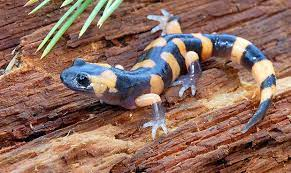
\includegraphics[scale=0.6]{sal}
		\vspace{4mm}
		
		두 타입의 도롱뇽 모집단: Rough Butt (R) and White Side (W)
		\vspace{3mm}
		
		$\surd$ Do salamanders prefer mating with their own population?
		\end{center}
		
		
	    \pagebreak
		
	    
		\textbf{실험계획} \\
		\vspace{4mm}
		\begin{itemize}
			\item 각 도롱뇽은 두 타입의 파트너와 모두 매칭됨 (반복 측정)
			\vspace{2mm}
			 \item 각 도롱뇽은 짝짖기에 대한 개별적인 성향을 가지고 있으며, 이는 측정할 수 없음
			\vspace{2mm}
			 \item 각 도롱뇽의 성향은 독립적이라고 가정
			\vspace{4mm}
			 
			 \item 도롱뇽이 짝짓기를 할 확률에 영향을 미치는 효과:
			 \begin{itemize}
			 	\item 페어링 타입 (RR, RW, WR, WW) (고정 효과)
			 	\item 암컷의 개별 짝짓기 성향 (랜덤 효과)
			 	\item 수컷의 개별 짝짓기 성향 (랜덤 효과)
			 \end{itemize}
		\end{itemize}
	
	\pagebreak
		\textbf{실험계획} \\
	\vspace{4mm}
	\begin{itemize}
		
		\item 반응변수: 짝짓기 유무 (Binary)
		\item 고정효과: $\beta_{RR}, \beta_{RW}, \beta_{WR}, \beta_{WW}$ (짝짓기 확률의 로그 오즈)
		\item 랜덤효과: 개별 성향 반영, 서로 독립이고 정규분포를 따른다고 가정
		\item 추정 분산: $\sigma_{F}^{2}, \sigma_{M}^{2}$
		
	\end{itemize}
	\vspace{5mm}
	
		$\triangleright$ How?


	\end{frame}
}


\section{Inference}{
		\begin{frame}[allowframebreaks]{Inference}
		\textbf{Likelihood based Inference}
		\vspace{4mm}
		
		\begin{itemize}
		\item $y_{i}=(y_{i1},...,y_{im_{i}}, U_{i})$의 결합 분포(Joint):
		
		\begin{center}
			$f(y_{i},U_{i};\beta,\theta)=f(U_{i};\theta)f(y_{i}|U_{i},\beta)=f(U_{i};\theta)\prod_{j=1}^{m_{i}} f(y_{ij}|U_{i},\beta)$
		\end{center}
		\vspace{2mm}
	
		\item $y_{i}$의 주변분포(Marginal):
		
		\begin{center}
			$f(y_{i},U_{i};\beta,\theta)=\int f(U_{i};\theta)\prod_{j=1}^{m_{i}} f(y_{ij}|U_{i},\beta)dU_{i}$
		\end{center}
	\vspace{2mm}
	
		\item 우도함수(Likelihood):
		
		\begin{center}
			$L(\beta,\theta; y)=\prod_{i=1}^{n}\lmoustache f(U_{i};\theta)\prod_{j=1}^{m_{i}} f(y_{ij}|U_{i},\beta)dU_{i}$	
		\end{center}
	
	\vspace{2mm}
	
	$y_{ij}$가 정규분포라면 위 적분의 계산이 비교적 간단한 반면, 대부분의 경우 closed form이 존재하지 않고 복잡해 일반적으로 랜덤 효과에 대해서 다변량 정규분포를 적용한다.
	\vspace{2mm}
	
	이 경우 크게 (1) \textbf{구적법}(Quadrature), (2) \textbf{몬테카를로}(Monte Carlo) 방법, (3) \textbf{우도함수의 근사화} 방법을 사용한다.
		\end{itemize}
	
		\pagebreak
		\textbf{수치적 방법: 구적법}
		\vspace{4mm}
		
		구적에 의한 근사화는 피적분함수의 가중치합(weighted sum)이다. 이때 여러가지 구적법 중 \textbf{Gauss-Hermite}(GHQ)와 \textbf{adaptive Gaussian}(AGQ) 구적법이 가장 많이 쓰인다.
		\vspace{2mm}
		
		\begin{center}
			$\int^{\infty}_{-\infty} e^{-x^{2}}f(x)dx \approx \sum^{R}_{k=1}w_{k}f(a_{k})$
		\end{center}
		
		\begin{itemize}
			\item 다항함수로 근사화될 수 있는 $f$에 대한 적분은 $R$개의 가중치합으로 근사화될 수 있으며, 여기서 $a_{k}$는 \textbf{구적점}(quadrature point), $w_{i}$는 \textbf{구적 가중치}(quadrature weight)라고 한다.
			\item GHQ 방법에서는 구적점이 고정된 반면, AGQ 방법에서는 구적접의 위치를 피적분 함수의 형태에 따라 변화시킴으로써 적분의 정확성을 향상시키고자 함
			\item SAS의 NLMIXED 모형의 경우, AGQ 방법 또는 1차 테일러 시리즈 근사를 통해 적분을 근사시킴
		\end{itemize}
	
	\pagebreak
	\textbf{우도함수의 근사화}
	\vspace{4mm}
	
	적분을 포함한 우도함수에 대해 \textbf{Laplace} 근사화를 적용할 수 있다.
	\vspace{2mm}
	
	\begin{center}
	\begin{align}
		\int^{\infty}_{-\infty} exp(f(x))dx & \approx \int^{\infty}_{-\infty} exp[{f(\tilde{x})-(x-\tilde{x})^{2}}/{2\sigma^{2}}]dx \\
		& =\int^{\infty}_{-\infty}exp(f({\tilde{x}}))\sqrt{2\pi}\sigma\phi(x;\tilde{x},\sigma^{2})dx \\ 
		& =exp(f(\tilde{x}))\sqrt{2\pi}\sigma \\
		& =c|f''(x)|^{-1/2}exp(f(\tilde{x}))
	\end{align}	
	\end{center}
	
	\begin{itemize}
		\item (3)은 $\phi(x;\tilde{x},\sigma^{2})$는 평균이 $\tilde{x}$이고 분산이 $\sigma^{2}$인 정규분포일때, $\tilde{x}$가 f(x)의 최빈값으로 $f'(\tilde{x})=0$이고 $f''(\tilde{x})=1/\sigma^{2}$임을 적용함
		\item 랜덤 효과가 정규분포를 따를 때만 적용할 수 있다.
	\end{itemize}
	\end{frame}}



\begin{frame}{Reference}
	\begin{thebibliography}{9}
		\bibitem{Alan} 
		Alan Agresti. 
		\textit{Categorical Data Analysis,Third Edition}. 
		Wiley. 2013.
		\bibitem{B} 
		Breslow, N. and Clayton, D.
		\textit{Approximate inference in generalized linear mixed models}. 
		Journal of the American Statistical Association. 88:9-25. 1993.
		\bibitem{C} 
		Christina Knudson. 
		\textit{Likelihood-Based Inference for Generalized Linear Mixed Models: Inference with R Package glmm}. 
		University of St. Thomas. 2017.
		\bibitem{J} 
		Jiming Jiang. 
		\textit{Linear and Generalized Linear Mixed Models and Their Applications}. 
		Springer. 2007.
		\bibitem{M} 
		M. Ataharul Islam.
		\textit{Analysis of Repeated Measures Data}. 
		Springer. 2017.
		\bibitem{K} 
		김양진.
		\textit{R과 SAS를 이용한 경시적 자료분석}. 
		자유아카데미. 2017.
	\end{thebibliography}
\end{frame}
\label{key}

\end{document}

